\documentclass[11pt,a4paper]{article} % Сурс - семинары по алгебре Медведя Никиты Юрьевича
\usepackage[utf8]{inputenc}
\usepackage[T2A]{fontenc}

\usepackage[english,russian]{babel}
\usepackage{amsfonts,amssymb}
\usepackage{graphicx}
\graphicspath{ {.} }

\usepackage{amsmath}
\usepackage{amsthm}
\usepackage{relsize}

\usepackage{systeme}

\usepackage{indentfirst} % Красная строка
\usepackage{fancyhdr}
\usepackage{wrapfig}
\usepackage{textcomp}

\usepackage{xcolor}% http://ctan.org/pkg/xcolor
%\usepackage{colortbl}% http://ctan.org/pkg/colortbl
\usepackage{multirow}% http://ctan.org/pkg/multirow
\usepackage{graphicx}% http://ctan.org/pkg/graphicx

\usepackage[unicode]{hyperref}

\usepackage{scontents}

% Blank formula checking
\usepackage{ifthen}
\newlength{\pheight}

\usepackage{centernot}
\usepackage{tabularx}
\usepackage{adjustbox, array, hhline}
\usepackage{makecell}

\addtolength{\textwidth}{114pt}
\addtolength{\hoffset}{-1cm}
\addtolength{\voffset}{-3cm}
\addtolength{\textheight}{170pt}

\tolerance=3000
% \flushbottom

\parindent=1cm

\begin{document}

\section*{Пункт 1.}

\def \flr#1{\left\lfloor #1 \right\rfloor}

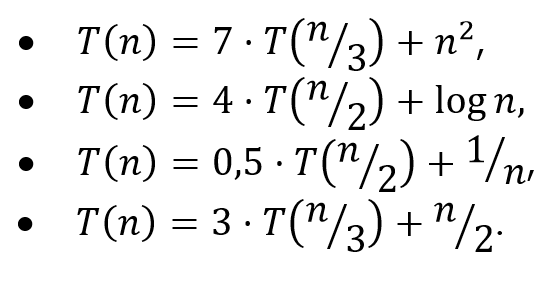
\includegraphics[scale=0.45]{alg21.png}

\begin{tabular}{l}
    $ 1. \hspace*{6pt} T(n) = 7 * T(\frac{n}{3}) + n^2 $ \\
    В данном случае $ a = 7 \ge 1 , b = 3 > 1. $ a и b не зависят от n. \\
    Дополнительная работа на каждом шаге рекурсии $ f(n) $ представима в виде \\
    $ f(n) = \Theta(n^{c}), \hspace*{6pt} c = 2. $ $ c $ не зависит от n, оценкой временной сложности $ f(n) $ \\
    является мономом $ \implies $ можно применить master-теорему. \\
    \\
    $ \log_b{a} = \log_3{7} < \log_3{9} = 2 = c \implies c > \log_b{a} $ \\
    $ (c > \log_b{a}) \wedge (f(n) = \Theta(n^{c})) \implies $ по второй формулировке master-теоремы \\
    $ T(n) = \Theta(n^{c}) = \Theta(n^{2}) $ \\
    \\
    Ответ: $ T(n) = \Theta(n^{2}) $ \\
    \\
\end{tabular}

\begin{tabular}{l}
    $ 2. \hspace*{6pt} T(n) = 4 * T(\frac{n}{2}) + \log n $ \\
    В данном случае $ a = 4 \ge 1, b = 2 > 1. $ a и b не зависят от n. \\
    Дополнительная работа на каждом шаге рекурсии $ f(n) $ представима в виде \\
    $ f(n) = \Theta(\log n) $ \\
    \\
    $ f(n) = \Theta(\log n) \implies f(n) = \mathcal{O}(\log n) \implies \forall k > 0: f(n) = \mathcal{O}(n^{k}) $ \\
    Положим $ k := 1 = 2 - 1 = \log_2 4 - 1 = \log_b a - 1 \implies $ по первой формулировке \\
    master-теоремы при $ \epsilon = 1 \hspace*{6pt} f(n) = \mathcal{O}(n^{\log_b a - \epsilon}) \implies T(n) = \Theta(n^{\log_b a}) = \Theta(n^2) $ \\
    \\
    Ответ: $ T(n) = \Theta(n^2) $ \\
    \\
\end{tabular}

\begin{tabular}{l}
    $ 3. \hspace*{6pt} T(n) = 0.5 * T(\frac{n}{2}) + \frac{1}{n} $ \\
    В данном случае $ a = 0.5 < 1 \implies $ применение master-теоремы невозможно. \\
    \\
    Ответ: применение master-теоремы невозможно, т.к. $ a = 0.5 < 1 $ \\
    \\
\end{tabular}

\begin{tabular}{l}
    $ 4. \hspace*{6pt} T(n) = 3 * T(\frac{n}{3}) + \frac{n}{2} $ \\
    В данном случае $ a = 3 \ge 1, b = 3 > 1. $ a и b не зависят от n. \\
    Дополнительная работа на каждом шаге рекурсии $ f(n) $ представима в виде \\
    $ f(n) = \Theta(n^{c}), \hspace*{6pt} c = 1. $ $ c $ не зависит от n, оценкой временной сложности $ f(n) $ \\
    является мономом $ \implies $ можно применить master-теорему. \\
    \\
    $ \log_a b = \log_3 3 = 1 = c \implies f(n) = \Theta(n^{\log_b a}) \implies $ по первой формулировке \\
    master-теоремы $ T(n) = \Theta(n^{\log_b a} \log n) = \Theta(n \log n) $ \\
    \\
    Ответ: $ T(n) = \Theta(n \log n) $ \\
    \\
\end{tabular}

\section*{Пункт 2.}

Master-теорема не применима для оценки функции временной сложности
$ T(n) = 0.5 * T(\frac{n}{2}) + \frac{1}{n} $

При помощи метода подстановки докажем, что $ \mathcal{O}(\log n) $ является
возможной асимптотически верхней границей данной функции временной сложности.

\begin{equation*}
\begin{split}
& T(n) = \mathcal{O}(\log n) \iff \left(
    \exists n_0 \in \mathbb{N} \hspace*{4pt} \exists c > 0 \hspace*{4pt} \forall n \ge n_0 \implies T(n) \le c \log_2 n
\right) \\
& \text{Покажем, что при } T(n) = \mathcal{O}(\log n) \hspace*{4pt}
    \exists n_0 \in \mathbb{N} \hspace*{4pt} \exists c > 0 \hspace*{4pt} \forall n \ge n_0 \implies
        0.5 * T\left(\frac{n}{2}\right) + \frac{1}{n} \le c \log_2 n \\ 
& 0.5 * T\left(\frac{n}{2}\right) + \frac{1}{n} \le 0.5 * c \log_2 \frac{n}{2} + \frac{1}{n} \le 0.5 * c \log_2 \frac{n}{2} + 1 \text{ при } n \ge 1 \\
& 0.5 * c \log_2 \frac{n}{2} + 1 = 0.5 * c \log_2 n - 0.5 c + 1 = 0.5 * c \log_2 n \text{ при } c = 2 \\
& \text{При } c > 0 \wedge n \in \mathbb{N} \implies 0.5 * c \log_2 n \le c \log_2 n \\
& \text{Получили: } ( n \ge 1 \wedge c = 2 \implies 0.5 * T\left(\frac{n}{2}\right) + \frac{1}{n} \le c \log_2 n ) \implies \\
& \exists n_0 = 1 \in \mathbb{N} \hspace*{4pt} \exists c = 2 > 0 \hspace*{4pt} \forall n \ge n_0 \implies T(n) \le c \log_2 n \\
& \text{Следовательно, } f(n) = \mathcal{O}(\log n) \\
& \hspace*{384pt} q.e.d. \\
& \text{Ответ: } T(n) = 0.5 * T\left(\frac{n}{2}\right) + \frac{1}{n} = \mathcal{O}(\log n) \\
\end{split}
\end{equation*}

\end{document}